\documentclass{article}
\usepackage{graphicx}
\usepackage{amsmath}
\usepackage{cite}

\begin{document}

\title{Higher dim Osc}


\maketitle


\section{Introduction}
We make the metric Ansatz: 
\begin{equation}
ds^2 = \alpha^2 dt^2+a^2 dr^2 + r^2 d\Omega_{3}
\end{equation}
where $A(t,r) = a^2$ and $C(t,r) = (a/\alpha)^2 $. \\  
The Einstein equation t,t component in 3+1D
\begin{equation}
    \label{KG Equation }
    \begin{split}
   A^{(0,1)}(t,r) & =\frac{1}{2} r A(t,r) \phi^{(1,0)}(t,r)^2 C(t,r)+\frac{1}{2} r A(t,r) \phi^{(0,1)}(t,r)^2+\frac{1}{2} r A(t,r)^2 \phi(t,r)^2 \\ &-\frac{1. A(t,r)^2}{r}+\frac{1. A(t,r)}{r}
	\end{split}
\end{equation}
The Einstein equation t,t component in 4+1D
\begin{equation}
\begin{split}
A^{(0,1)}(t,r)&=\frac{1}{3} r A(t,r) \phi^{(1,0)}(t,r)^2 C(t,r)+\frac{1}{3}r A(t,r) \phi^{(0,1)}(t,r)^2+\frac{1}{3} r A(t,r)^2 \phi(t,r)^2 \\ &-\frac{2. A(t,r)^2}{r}+\frac{2. A(t,r)}{r}
	\end{split}
\end{equation}
The Einstein equation t,r component in 3+1D
\begin{equation}
A^{(1,0)}(t,r)=r A(t,r) \phi^{(0,1)}(t,r) \phi^{(1,0)}(t,r)
\end{equation}
The Einstein equation t,r component in 4+1D
\begin{equation}
A^{(1,0)}(t,r)=\frac{2}{3} r A(t,r) \phi^{(0,1)}(t,r) \phi^{(1,0)}(t,r)
\end{equation}
The Einstein equation r,r component in 3+1D
\begin{equation}
\begin{split}
C^{(0,1)}(t,r)=  r A(t,r) \phi(t,r)^2 C(t,r)-\frac{2. A(t,r) C(t,r)}{r}+\frac{2. C(t,r)}{r}
\end{split}
\end{equation}
The Einstein equation r,r component in 4+1D
\begin{equation}
\begin{split}
C^{(0,1)}(t,r)=\frac{2}{3} r A(t,r) \phi(t,r)^2 C(t,r)-\frac{4. A(t,r) C(t,r)}{r}+\frac{4. C(t,r)}{r}
\end{split}
\end{equation}
The Klein Gordon equation in 3+1D in as similar form as the paper
\begin{equation}
\begin{split}
\phi^{(2,0)}(t,r) C(t,r)&=-\frac{C^{(0,1)}(t,r) \phi^{(0,1)}(t,r)}{2 C(t,r)}-A(t,r) \phi(t,r)\\&-\frac{1}{2} C^{(1,0)}(t,r) \phi^{(1,0)}(t,r)+\frac{2 \phi^{(0,1)}(t,r)}{r}+\phi^{(0,2)}(t,r)
\end{split}
\end{equation}
The Klein Gordon equation in 4+1D in as similar form as the paper
\begin{equation}
\begin{split}
\phi^{(2,0)}(t,r) C(t,r)&=-\frac{C^{(0,1)}(t,r) \phi^{(0,1)}(t,r)}{2 C(t,r)}-A(t,r) \phi(t,r)\\&-\frac{1}{2} C^{(1,0)}(t,r) \phi^{(1,0)}(t,r)+\frac{3 \phi^{(0,1)}(t,r)}{r}+\phi^{(0,2)}(t,r)
\end{split}
\end{equation}

The Klein Gordon equation in 3+1D in as similar form as the Code
\begin{equation}
\begin{split}
\phi^{(2,0)}(t,r) C(t,r)&=-0.5 r A(t,r) \phi^{(0,1)}(t,r) \phi(t,r)^2
\\ &+\frac{1. A(t,r) \phi^{(0,1)}(t,r)}{r}-A(t,r) \phi(t,r)-\frac{1}{2} C^{(1,0)}(t,r) \phi^{(1,0)}(t,r)
\\ &+\frac{1. \phi^{(0,1)}(t,r)}{r}+\phi^{(0,2)}(t,r)+0.
\end{split}
\end{equation}
The Klein Gordon equation in 4+1D in as similar form as the Code
\begin{equation}
\begin{split}
\phi^{(2,0)}(t,r) C(t,r)&=-\frac{1}{3} r A(t,r) \phi^{(0,1)}(t,r) \phi(t,r)^2
\\ &+\frac{2. A(t,r) \phi^{(0,1)}(t,r)}{r}-A(t,r) \phi(t,r)-\frac{1}{2} C^{(1,0)}(t,r) \phi^{(1,0)}(t,r)
\\ &+\frac{1. \phi^{(0,1)}(t,r)}{r}+\phi^{(0,2)}(t,r)+0.
\end{split}
\end{equation}
\section{Axion equation }
The Einstein equation t,t component in 3+1D
\begin{equation}
    \label{KG Equation }
    \begin{split}
A^{(0,1)}(t,r)&=\frac{1}{2} r A(t,r) \phi^{(1,0)}(t,r)^2 C(t,r)+\frac{1}{2} r A(t,r) \phi^{(0,1)}(t,r)^2+r A(t,r)^2 V(\phi(t,r))
\\&-\frac{A(t,r)^2}{r}+\frac{A(t,r)}{r}
	\end{split}
\end{equation}
The Einstein equation t,r component in 3+1D
\begin{equation}
\begin{split}
A^{(1,0)}(t,r)=r A(t,r) \phi^{(0,1)}(t,r) \phi^{(1,0)}(t,r)
\end{split}
\end{equation}
The Einstein equation r,r component in 3+1D
\begin{equation}
\begin{split}
C^{(0,1)}(t,r)=2 r A(t,r) V(\phi(t,r)) C(t,r)-\frac{2 A(t,r) C(t,r)}{r}+\frac{2 C(t,r)}{r}
\end{split}
\end{equation}
The Klein Gordon equation in 3+1D as in Paper 
\begin{equation}
\begin{split}
\phi^{(2,0)}(t,r) C(t,r)&=-\frac{C^{(0,1)}(t,r) \phi^{(0,1)}(t,r)}{2 C(t,r)}-A(t,r) V'(\phi(t,r))
\\&-\frac{1}{2} C^{(1,0)}(t,r) \phi^{(1,0)}(t,r)+\frac{2 \phi^{(0,1)}(t,r)}{r}+\phi^{(0,2)}(t,r)
\end{split}
\end{equation}
The Klein Gordon equation in 3+1D as in Code 
\begin{equation}
\begin{split}
\phi^{(2,0)}(t,r) C(t,r)&=-r A(t,r) \phi^{(0,1)}(t,r) V(\phi(t,r))\\&+\frac{A(t,r) \phi^{(0,1)}(t,r)}{r}-A(t,r) V'(\phi(t,r))-\frac{1}{2} C^{(1,0)}(t,r) \phi^{(1,0)}(t,r)
\\&+\frac{\phi^{(0,1)}(t,r)}{r}+\phi^{(0,2)}(t,r)
\end{split}
\end{equation}

\section{Fourier Space }

\begin{equation}
\phi(t,x) = \sum_{j = 0} ^{\infty} \hat{\phi}_j(x)\cos(j\omega t)
\end{equation}
\begin{equation}
A(t,x) = \sum_{j = 0} ^{\infty} \hat{A}_j(x)\cos(j\omega t)
\end{equation}
\begin{equation}
C(t,x) = \sum_{j = 0} ^{\infty} \hat{C}_j(x)\cos(j\omega t)
\end{equation}

\begin{equation}
\begin{split}
\phi(t,x) A(t,x) &= \sum_{j = 0} ^{\infty}\sum_{i = 0} ^{\infty} \hat{\phi}_j(x)\hat{A}_i(x)\cos(i\omega t)\cos(j\omega t) \\
&=  \sum_{n = 0} ^{\infty}\sum_{i = 0}^{\infty}\hat{\phi}_{n-i}(x)A_i(x)\frac{1}{2}(\cos((j+i)\omega t)+\cos((j-i)\omega t))\\
& \underbrace{=}_{n = i+j } \sum_{n = 0} ^{\infty}\sum_{i = 0}^{\infty} \hat{\phi}_{n-i}(x)\hat{A}_i(x)\frac{1}{2}(\cos(n\omega t)+\cos((j-i)\omega t))\\
& =  \sum_{n = 0} ^{\infty}\sum_{i = 0}^{\infty} \hat{\phi}_{n-i}(x)\hat{A}_{i}(x)\frac{1}{2}(\cos(n\omega t))+ \sum_{n = 0} ^{\infty}\sum_{i = 0}^{-\infty} \hat{\phi}_{n+i}(x)\hat{A}_{-i}(x)\frac{1}{2}(\cos(n\omega t))\\
& =  \sum_{n = 0} ^{\infty}\sum_{i = -\infty}^{\infty} \hat{\phi}_{n-|i|}(x)\hat{A}_{|i|}(x)\cos(n\omega t)
\end{split}
\end{equation}

will be written as
\begin{equation}
\begin{split}
 A(t,x) &= \sum_{j = 0} ^{\infty} \hat{A}_j(x)\partial_t\cos(j\omega t)= \sum_{j = 0} ^{\infty} \hat{A}_j(x)j\omega\cos(j\omega t) 
\end{split}
\end{equation}
\begin{equation}
    \label{KG Equation }
    \begin{split}
   A^{(0,1)}(t,r) & =\frac{1}{2} r A(t,r) \phi^{(1,0)}(t,r)^2 C(t,r)+\frac{1}{2} r A(t,r) \phi^{(0,1)}(t,r)^2+\frac{1}{2} r A(t,r)^2 \phi(t,r)^2 \\ &-\frac{1. A(t,r)^2}{r}+\frac{1. A(t,r)}{r}
	\end{split}
\end{equation}
In Fourier space 
\begin{equation}
    \label{KG Equation }
    \begin{split}
   \hat{A}_j^{(0,1)}(t) & =\frac{1}{2} r j^2\omega^2 (\hat{A} * \hat{\phi} * \hat{\phi} * \hat{C})_j+\frac{1}{2} r (\hat{A}*\hat{\phi}^{(0,1)}*\hat{\phi}^{(0,1)})_j+\frac{1}{2} r (\hat{A}*\hat{A} *\hat{\phi}*\hat{\phi})_j \\ &-\frac{(\hat{A}*\hat{A})_j}{r}+\frac{A_j}{r}
	\end{split}
\end{equation}

\section{ADM mass}
Asymptotic behaviour of Metric
\begin{equation}
ds^2 = -\left(A-\frac{2M}{r^{d-3}}\right)dt^2+\left(C-\frac{2M}{r^{d-3}}\right)^{-1}+r^2d\Omega_{d-2}^2
\end{equation}
where $C,B \in R $ we can find the asymptomatic mass by : 
\begin{equation}
\begin{split}
A &= \left(C-\frac{2M}{r^{d-3}}\right)^{-1} \\
M &= \frac{1}{2} \left(C - \frac{1}{A} \right) r^{-3 + d}
\end{split}
\end{equation} 

\section{Non-relativistic limit}

\begin{equation}
i \hbar \partial_t \psi = - \frac{\hbar^2}{2m}\nabla^2 \psi + m U \psi
\end{equation}
\begin{equation}
\nabla^2 U = 4 \pi G | \psi |^2
\end{equation}
we Fourier transform $\nabla = 1/L$ where L is the characteristic length of the Osc. 

\begin{equation}
i \hbar \partial_t \psi = - \frac{\hbar^2}{2m}\nabla^2 \psi + m U \psi
\end{equation}
\begin{equation}
\nabla^2 U = 4 \pi G | \psi |^2
\end{equation}
\section{Conclusion}
3+1D $\neq$ 4+1D

\section{AdS Solitons }

\subsection{Ansatz}

We make the metric Ansatz: 
\begin{equation}
ds^2 = \left(\alpha^2 - \frac{r^2\Lambda}{6}\right) dt^2+a^2dr^2 + r^2 d\Omega_{3}
\end{equation}
where $A(t,r) = a^2$ and $C(t,r) = (a/\alpha)^2 $. \\  

compared to the ansatz in BRITO PROCA Star

\begin{equation}
ds^2 = \sigma^2(r)F(r)dt^2+ \frac{1}{F(r)}dr^2+r^2d\Omega
\end{equation}
where $F(r) = 1 - \frac{2 m(r)}{r^2}-\Lambda r^2/6$  

\subsection{Stability}
In this section we discuss solution for higher-dimensional scalar and vector Boson stars \cite{Duarte:2016lig}. One finds that the maximum mass for Boson Stars in 5 dimension diverges for $\phi_0(0) \rightarrow 0 $. The biding energy seems to be negative for all values, indicating that such solution are unstable (analogous for Boson Stars: \cite{Brihaye:2015jja}). In \cite{Duarte:2016lig} they hypothise that for $\Lambda < 0$ there are stable solutions.  

\begin{figure}
  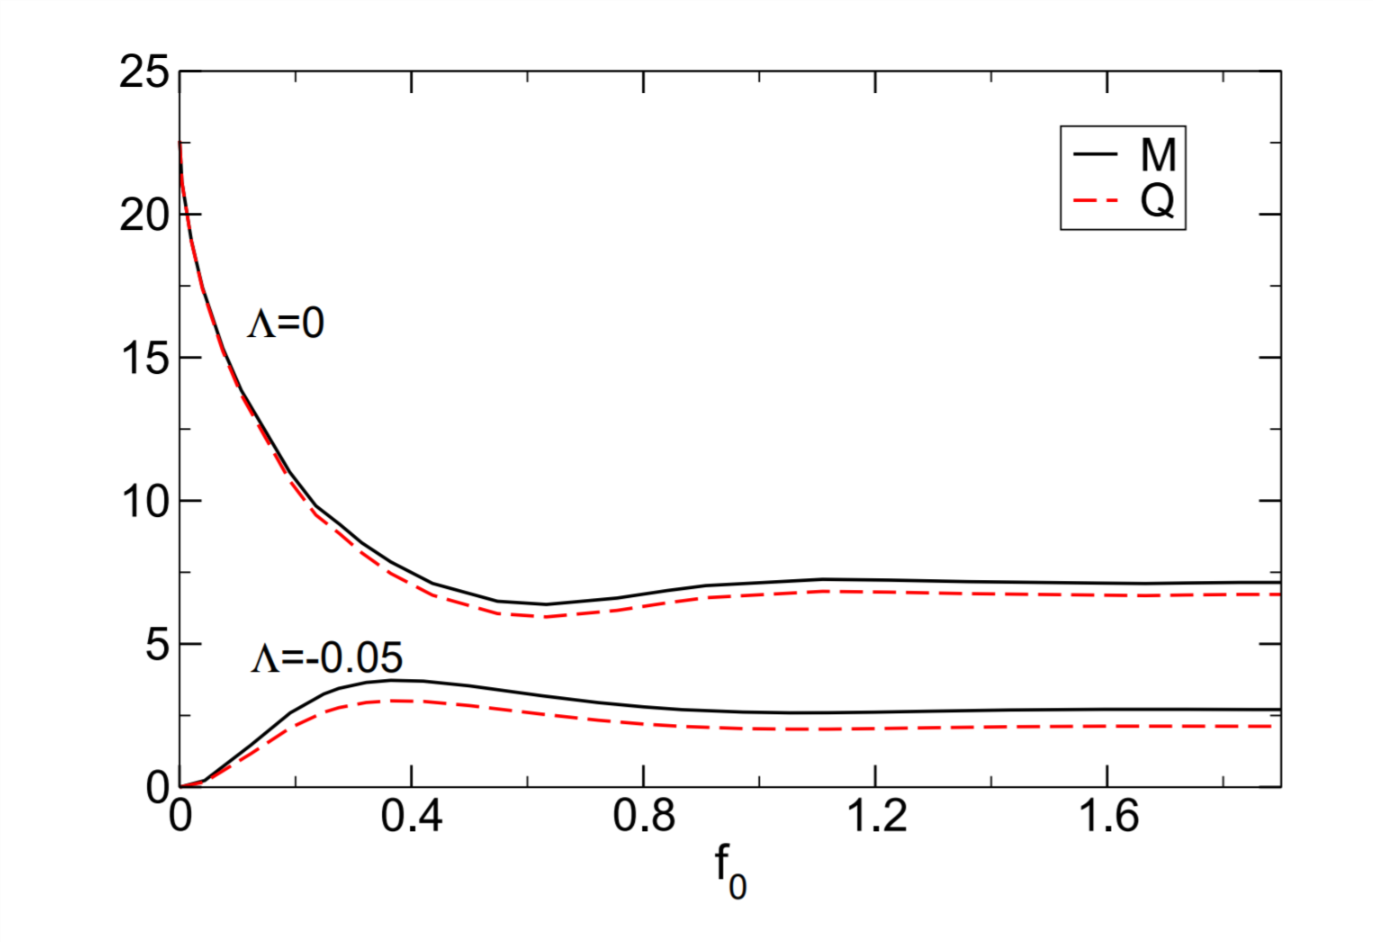
\includegraphics[width=\linewidth]{StabileADs.png}
	\caption{{\bf Stability of vector Boson stars in 5 dimension:} Where $f_0$ is the parameter defining Proca stars. Adding a negative cosmological constant gives the upper mass a bound.  }
  \label{fig:boat1}
\end{figure}

\bibliography{mybib}{}
\bibliographystyle{plain}
\end{document}
